% So we make this "beamer" rather than document! 

\documentclass[handout]{beamer}
\usetheme{default}
\usecolortheme{beaver}
\setbeamertemplate{navigation symbols}{}

\usepackage{beamerfoils}
%\usepackage{natbib} 
\usepackage[natbib=true, bibstyle=authoryear, citestyle=authoryear-comp]{biblatex}
\usepackage{graphicx} 
%\usepackage{geometry}
\bibliography{/Users/Nick/Dropbox/Dropbox_Documents/my_library}
%\bibliographystyle{apalike}
\usepackage{pgfpages}
\pgfpagesuselayout{2 on 1}[ shrink=5mm]

%\setbeameroption{show notes}
%\setbeamertemplate{note page}[plain]

\title{Understanding Private School Performance in Rural Pakistan}
\author{Nick Eubank}
\date{\today}


% This is the beginning of a real document!
\begin{document} 

\begin{frame}{}
	\titlepage
\end{frame}

\begin{frame}{Context}
Explosion of Rural Private Schools
	\begin{itemize}
		\item Pakistan: from 2000 to 2005, enrollment increased 47\%. \\ 
			By 2005, 1/3 of students in private school.
		\item India: in 2005, $>$20\% of rural students in private school.
	\end{itemize}
\pause
Private schools radically outperform government schools.
	\begin{itemize}
		\item \citep{Jimenez:1991wa, Jimenez:1995vg, Pratham:2005vw, Andrabi:2011hl, Desai:2009ty, Tooley:2003vf, Alderman:2003we, Alderman:2001wk}
	\end{itemize}	
\pause
But why?
\end{frame}

\begin{frame}{Explanation 1: Sorting}
	\begin{itemize}
		\item Even after controlling for HH wealth and parental education, maybe private school students are ``different.''
		\pause
		\begin{itemize}
			\item $>$20\% of households send send children to \emph{both} government and private schools. 
		\end{itemize}
		\item Some Attempts to control through randomization of vouchers
			\begin{itemize}
				\item \citep{Angrist:2002up, Bellei:2008uu}
			\end{itemize}
		\item But lots of problems...
			\begin{itemize}
				\item Risk of losing vouchers induces efforts
				\item Selective admission
			\end{itemize}
	\end{itemize}	
\pause
If true, then private school superiority is illusory. 
\end{frame}


\begin{frame}{Explanation 2: Better Incentives for Good Teachign}
What matters is not inputs, but effort
	\begin{itemize}
		\item Shown in the US: \cite{Hanushek:1997tt,Hanushek:2003hz,Banerjee:2007wx}
		\item Shown to be lacking in Government Schools in South Asia: \\
		\citep{Muralidharan:2008tb, Chaudhury:2006vp}
	\end{itemize}
\end{frame}

\begin{frame}{Contribution}
	Examines compatibility with novel finding: \\
	Private school dominance declines by 50\% with village caste fractionalization.
	\pause
	\begin{itemize}
		\item Consistent with private school dominance arising from selective ``sorting''
	\end{itemize}
\end{frame}

\begin{frame}{Why do we care?}
Vouchers: hope for the future, or waste of resources?
\begin{itemize}
	\item Big push: \citep{Chakrabarti:2008vc, Kelkar:2006tq, Panagariya:2008wi}
\end{itemize}
\pause
Model for Government Schools?
\begin{itemize}
	\item Stop hiring well educated teachers, instead focus on incentives.
\end{itemize}
\pause
We are literally talking about the education of \emph{hundreds of millions of children}.
\end{frame}


\section{Methodology}\label{}
\begin{frame}{Outline}
	\tableofcontents[currentsection]
\end{frame}

\begin{frame}{Data}	
Learning and Educational Attainment in Punjab Schools (LEAPS)
\begin{itemize}
	\item 2003-2007 panel data
	\item One four year panel (12,110 children)
	\item One two year panel (11,852 children)
	\item 112 Villages
	\item Three Districts
	\item Includes: Child Test Scores, Teacher Test Scores, Parental Educational, HH Wealth
	\item Test scores are normalized using IRT -- mean 0, standard deviation 1.
\end{itemize}
\end{frame}

\begin{frame}{Measuring Learning}
	Lagged-Value-Added Model:	
	\begin{eqnarray}
		Y_{i,t}=\alpha_tX_{i,t}+\alpha_{t-1}X_{i,t-1}+ \dots + \alpha_1X_{i,1} + \epsilon_{i,t}
	\end{eqnarray}
	\pause
	\begin{eqnarray}
		Y_{i,t}=X_{i,t}\alpha+Y_{i,t-1}\beta + \epsilon_{i,t}\label{primary}
	\end{eqnarray}
	\begin{itemize}
		\item Controls for differences in initial levels, but not differences in rates. 
		\item Flexible persistence parameter
		\item All past scores included to control of measurement error.
	\end{itemize}
\end{frame}

\begin{frame}{Measuring Learning}
	Village Level:
	\begin{enumerate}
		\item Run Lagged-Value Added regressions with village-school type dummies for each village $j$.
		\begin{eqnarray*}
			Y_{i,t}=X_{i,t}\alpha+Y_{i,t-1}\beta + \mathbb{I}_{i,j,type,t}\gamma_{j, type}+\epsilon_{i,t}
		\end{eqnarray*}
		\item Extract dummies and calculate village public-private gap.
		\item Analyze at level of village.
	\end{enumerate}
	\begin{eqnarray*}
		Gap_{j}=Z_{j}\delta+\eta_{j}\label{villagespecification}
	\end{eqnarray*}
\end{frame} 

\begin{frame}{Measuring Learning}
	Teacher Level:
	\begin{enumerate}
		\item Run Lagged-Value Added regressions with teacher fixed effects dummies for each teacher $k$.
		\begin{eqnarray*}
			Y_{i,t}=X_{i,t}\alpha+Y_{i,t-1}\beta + \mathbb{I}_{i,k,t}\zeta_{k}+\epsilon_{i,t}\label{teacherspecification}
		\end{eqnarray*}
		
		\item Extract fixed effect coefficients as estimates of teacher contributions
		\item Analyze at level of teacher (weighted by number of students).
	\end{enumerate}
\end{frame}


\section{Fractionalization and Performance}\label{}
\begin{frame}{Outline}
	\tableofcontents[currentsection]
\end{frame}

\begin{frame}{Caste in Punjab}
\begin{itemize}
	\item Very similar to caste in India
	\begin{itemize}
		\item Biraderi implies ``an inherent, inbuilt hierarchy that governs social interactions''\citep[p. 29]{Gazdar:2007vt}.	
	\end{itemize}
	\item Not synonymous with economic status:
	\begin{itemize}
		\item ``the poorest Jatt is still better off than the richest kammi.'' \citep[p. 13]{Gazdar:2007vt} 
	\end{itemize}
\end{itemize}
\end{frame}
	
\begin{frame}{Caste in Punjab}
	\begin{figure}[htb]
		\begin{center}
		\label{fracdensities}
		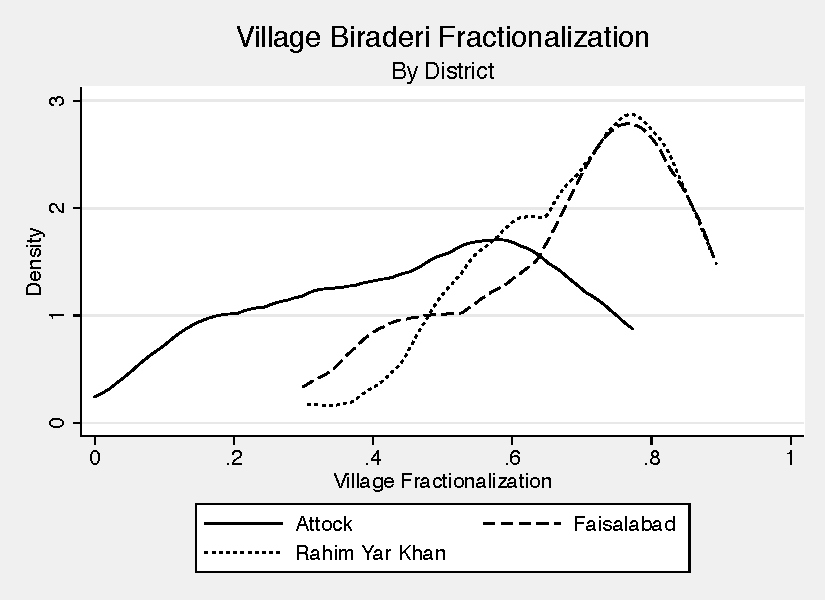
\includegraphics[scale=0.6]{graphs/village_frac_by_district.pdf}
		\end{center}
	\end{figure}		
\end{frame}

\begin{frame}{Caste in Punjab}
	% Note really correlated with stuff
\end{frame}

\begin{frame}{Caste Fractionalization and Test Scores}
	\begin{figure}[h]
		\caption{Private School Test Score Premium with Lagged Scores}\label{kidscombined}
		\centering	
		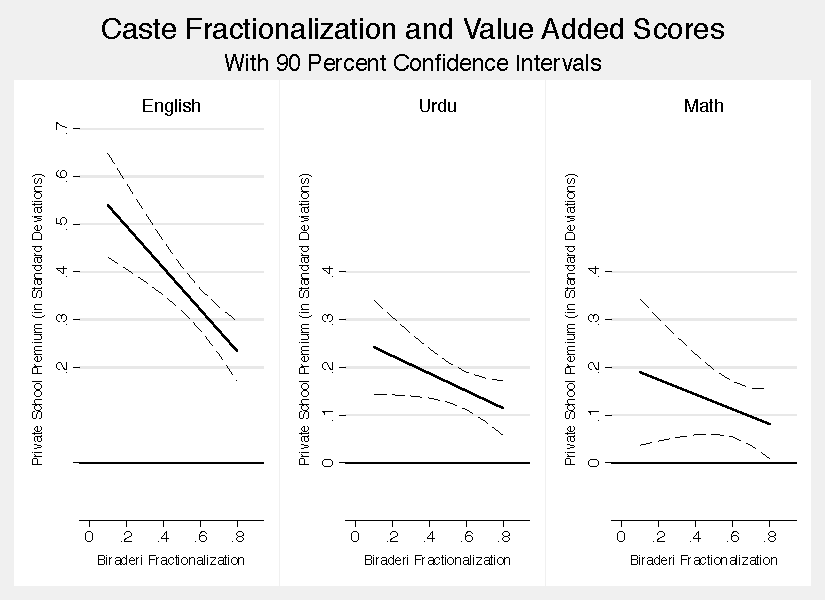
\includegraphics[scale=0.8]{graphs/kids_combined.pdf}
	\end{figure}
\end{frame}

\begin{frame}{Caste Fractionalization and Test Scores}
	% \begin{table}[htbp]\centering
\def\sym#1{\ifmmode^{#1}\else\(^{#1}\)\fi}
\caption{Village Level Government-Private Gap\label{villagegap}}
\begin{tabular}{l*{3}{c}}
\toprule
                &\multicolumn{1}{c}{(1)}&\multicolumn{1}{c}{(2)}&\multicolumn{1}{c}{(3)}\\
                &\multicolumn{1}{c}{English}&\multicolumn{1}{c}{Urdu}&\multicolumn{1}{c}{Math}\\
\midrule
Biraderi Fractionalization&    -0.36*  &    -0.18   &    -0.28   \\
                &  (-1.80)   &  (-1.02)   &  (-1.03)   \\
Median Village Wealth&-0.000010   &0.0000096   &-0.000043   \\
                &  (-0.32)   &   (0.34)   &  (-0.97)   \\
Log Village Size&   0.0016   &   -0.033   &    0.019   \\
                &   (0.03)   &  (-0.63)   &   (0.23)   \\
Pct of Adults Literate& -0.00021   &   0.0019   &   0.0047   \\
                &  (-0.06)   &   (0.64)   &   (1.00)   \\
Land Gini       &     0.35   &   -0.084   &     0.32   \\
                &   (1.01)   &  (-0.27)   &   (0.66)   \\
District Fixed Effects&      Yes   &      Yes   &      Yes   \\
\midrule
Observations    &      109   &      109   &      109   \\
\bottomrule
\multicolumn{4}{l}{\footnotesize \textit{t} statistics in parentheses}\\
\multicolumn{4}{l}{\footnotesize * p<0.10, ** p<0.05, *** p<0.01}\\
\end{tabular}
\end{table}

\end{frame}

\section{School Quality}\label{}
\begin{frame}{Outline}
	\tableofcontents[currentsection]
\end{frame}

\begin{frame}{No Difference in Inputs}
	\begin{figure}[htb]
		\begin{center}
		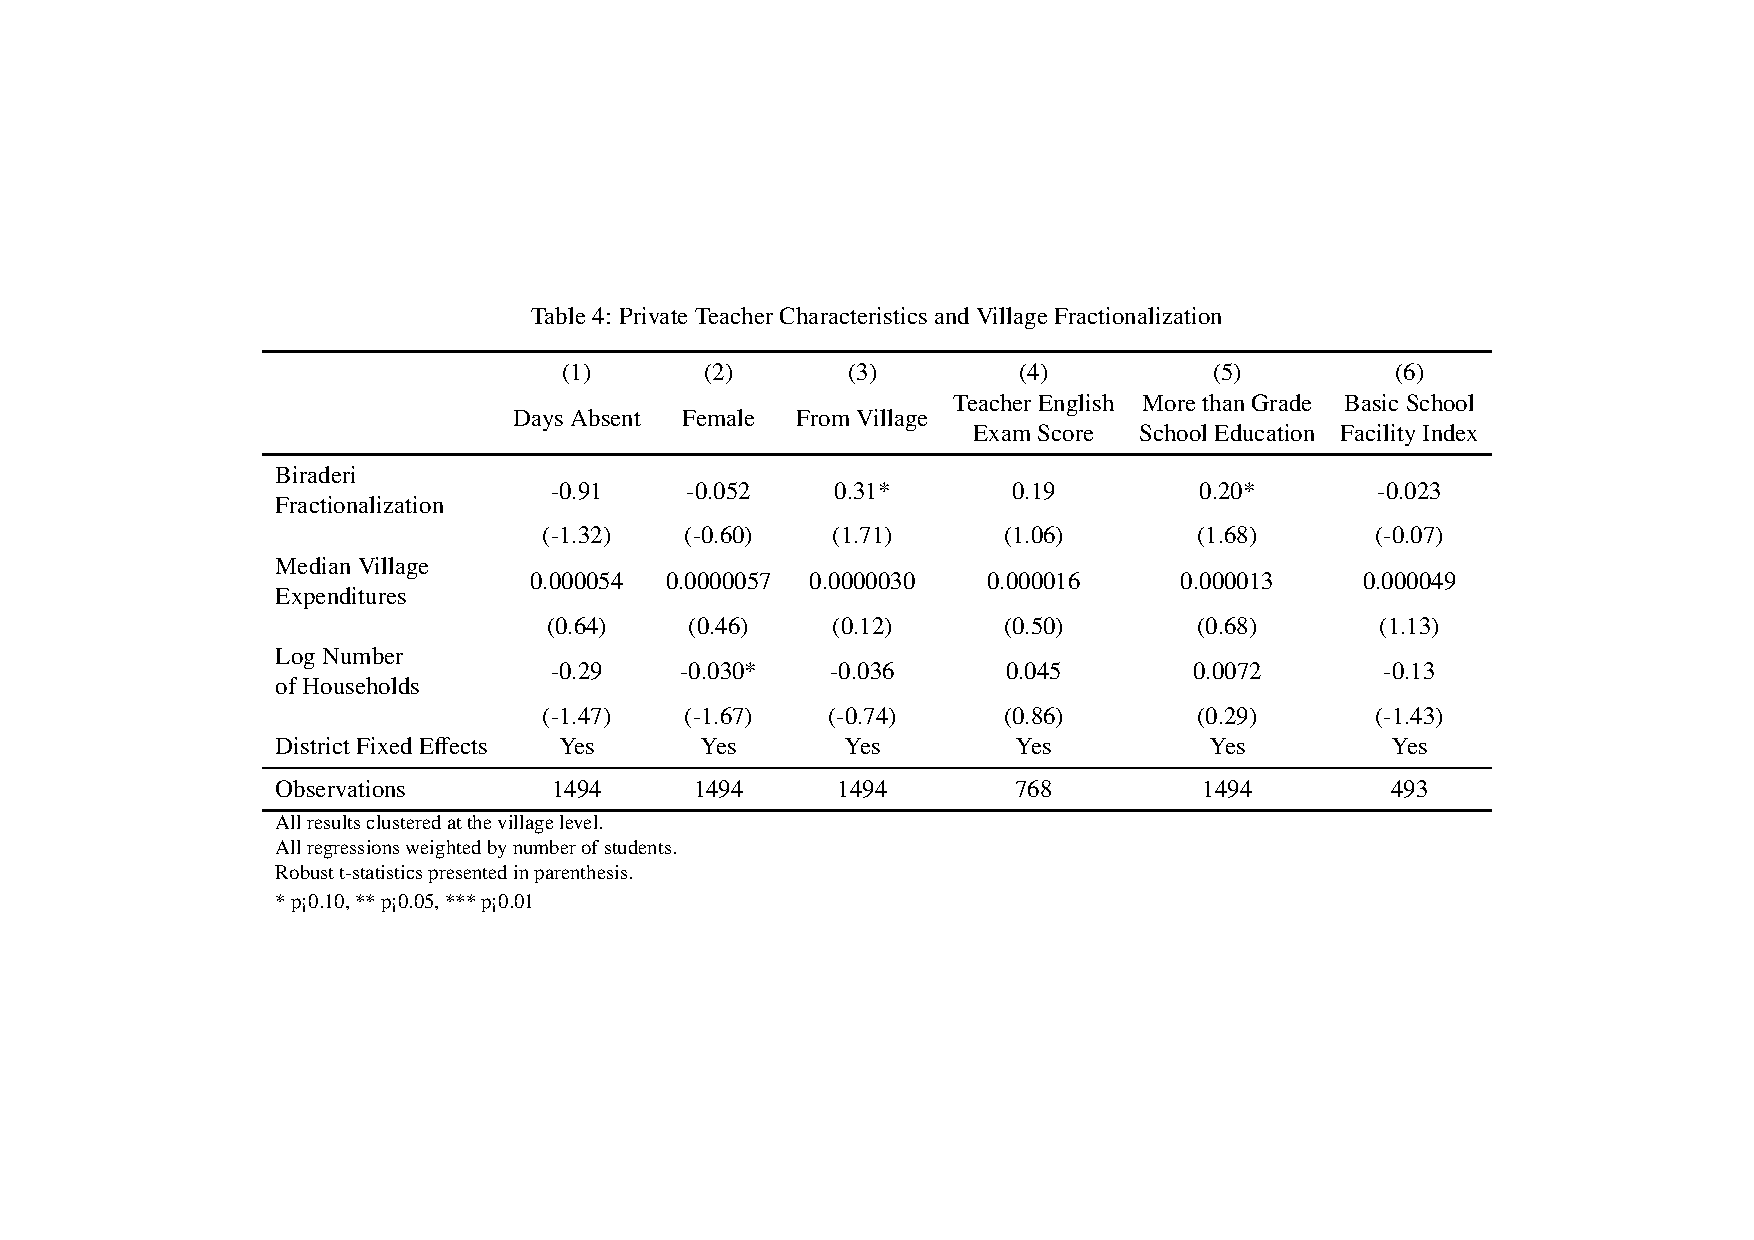
\includegraphics[scale=0.5]{tables/Private_teacher_quality.pdf}
		\end{center}
	\end{figure}
\end{frame}

\begin{frame}{No Difference in Inputs}
	\begin{figure}[htb]
		\begin{center}
		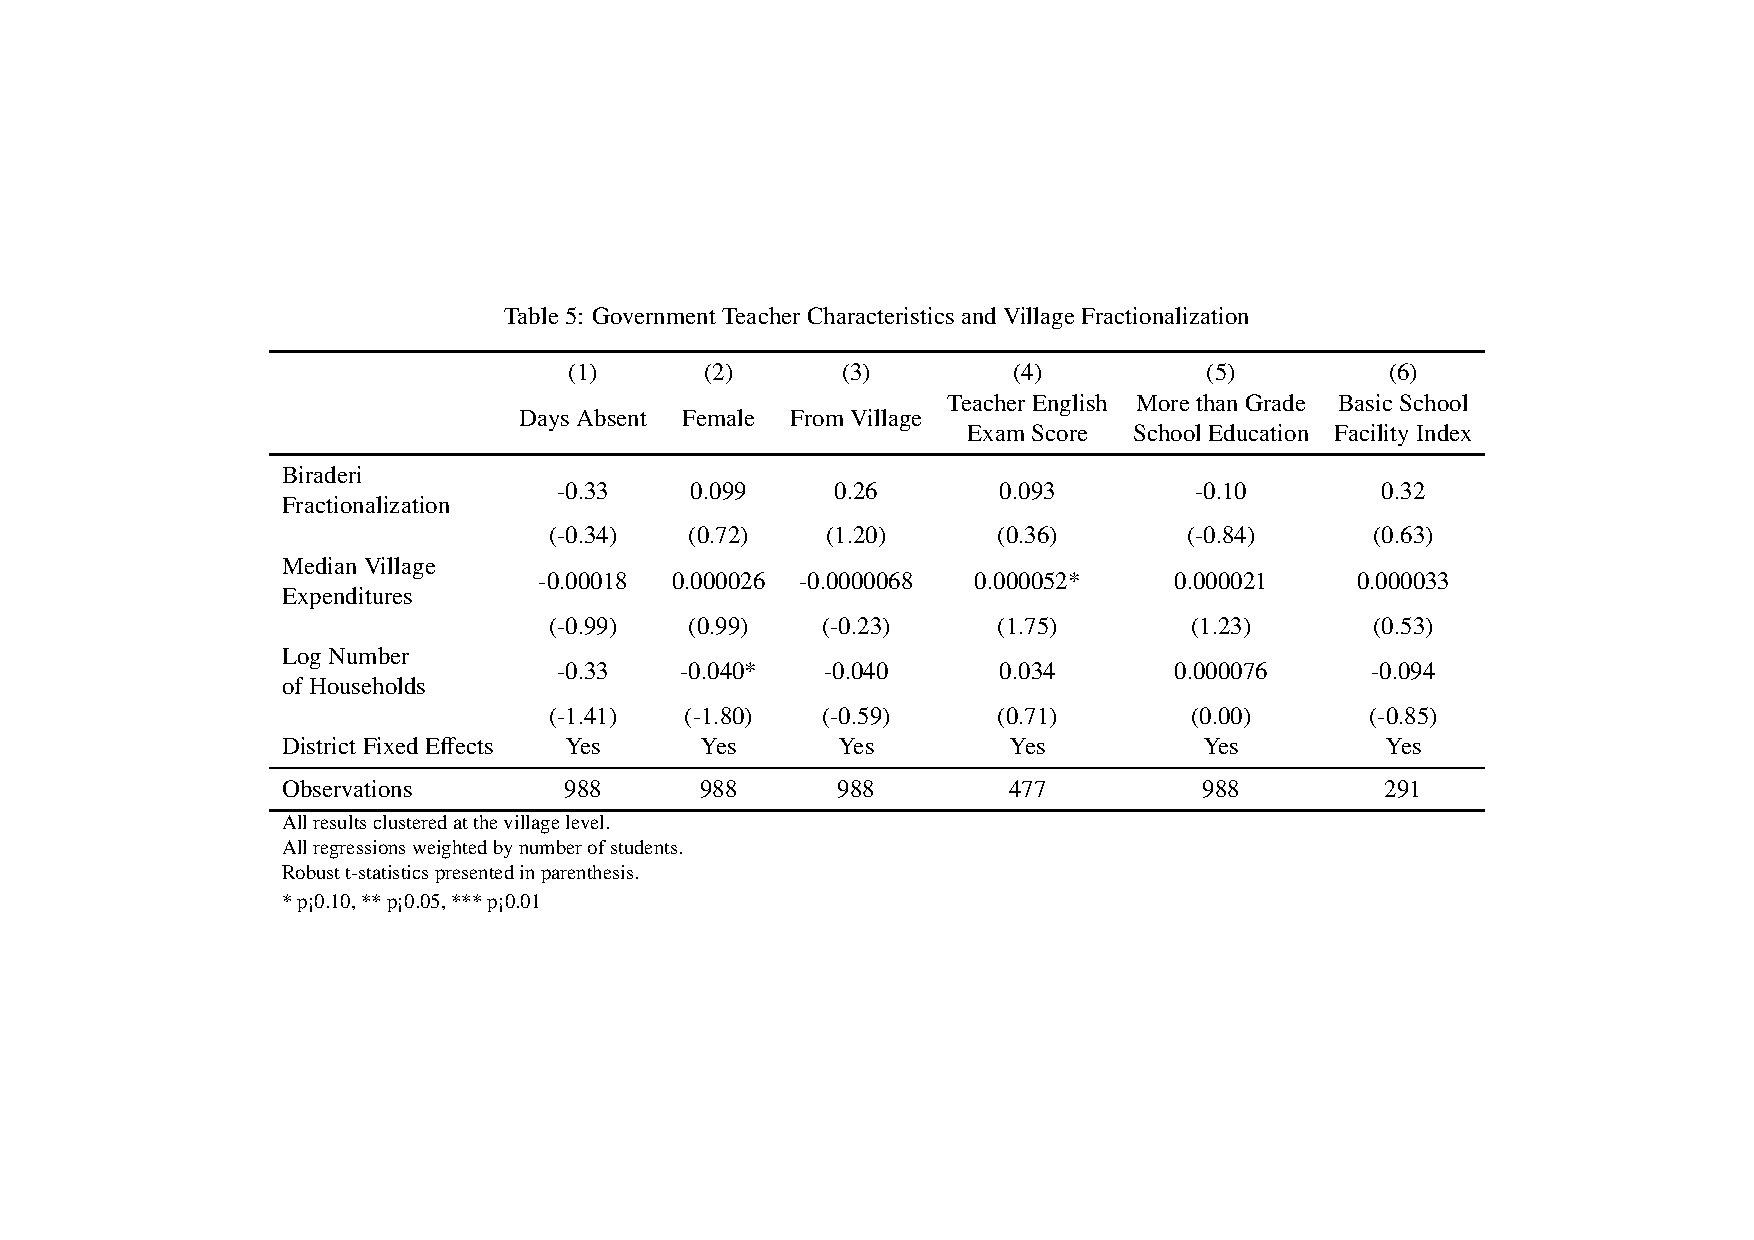
\includegraphics[scale=0.5]{tables/govt_teacher_quality.pdf}
		\end{center}
	\end{figure}
	
\end{frame}

\begin{frame}{}
	\begin{figure}[htb]
		\begin{center}
		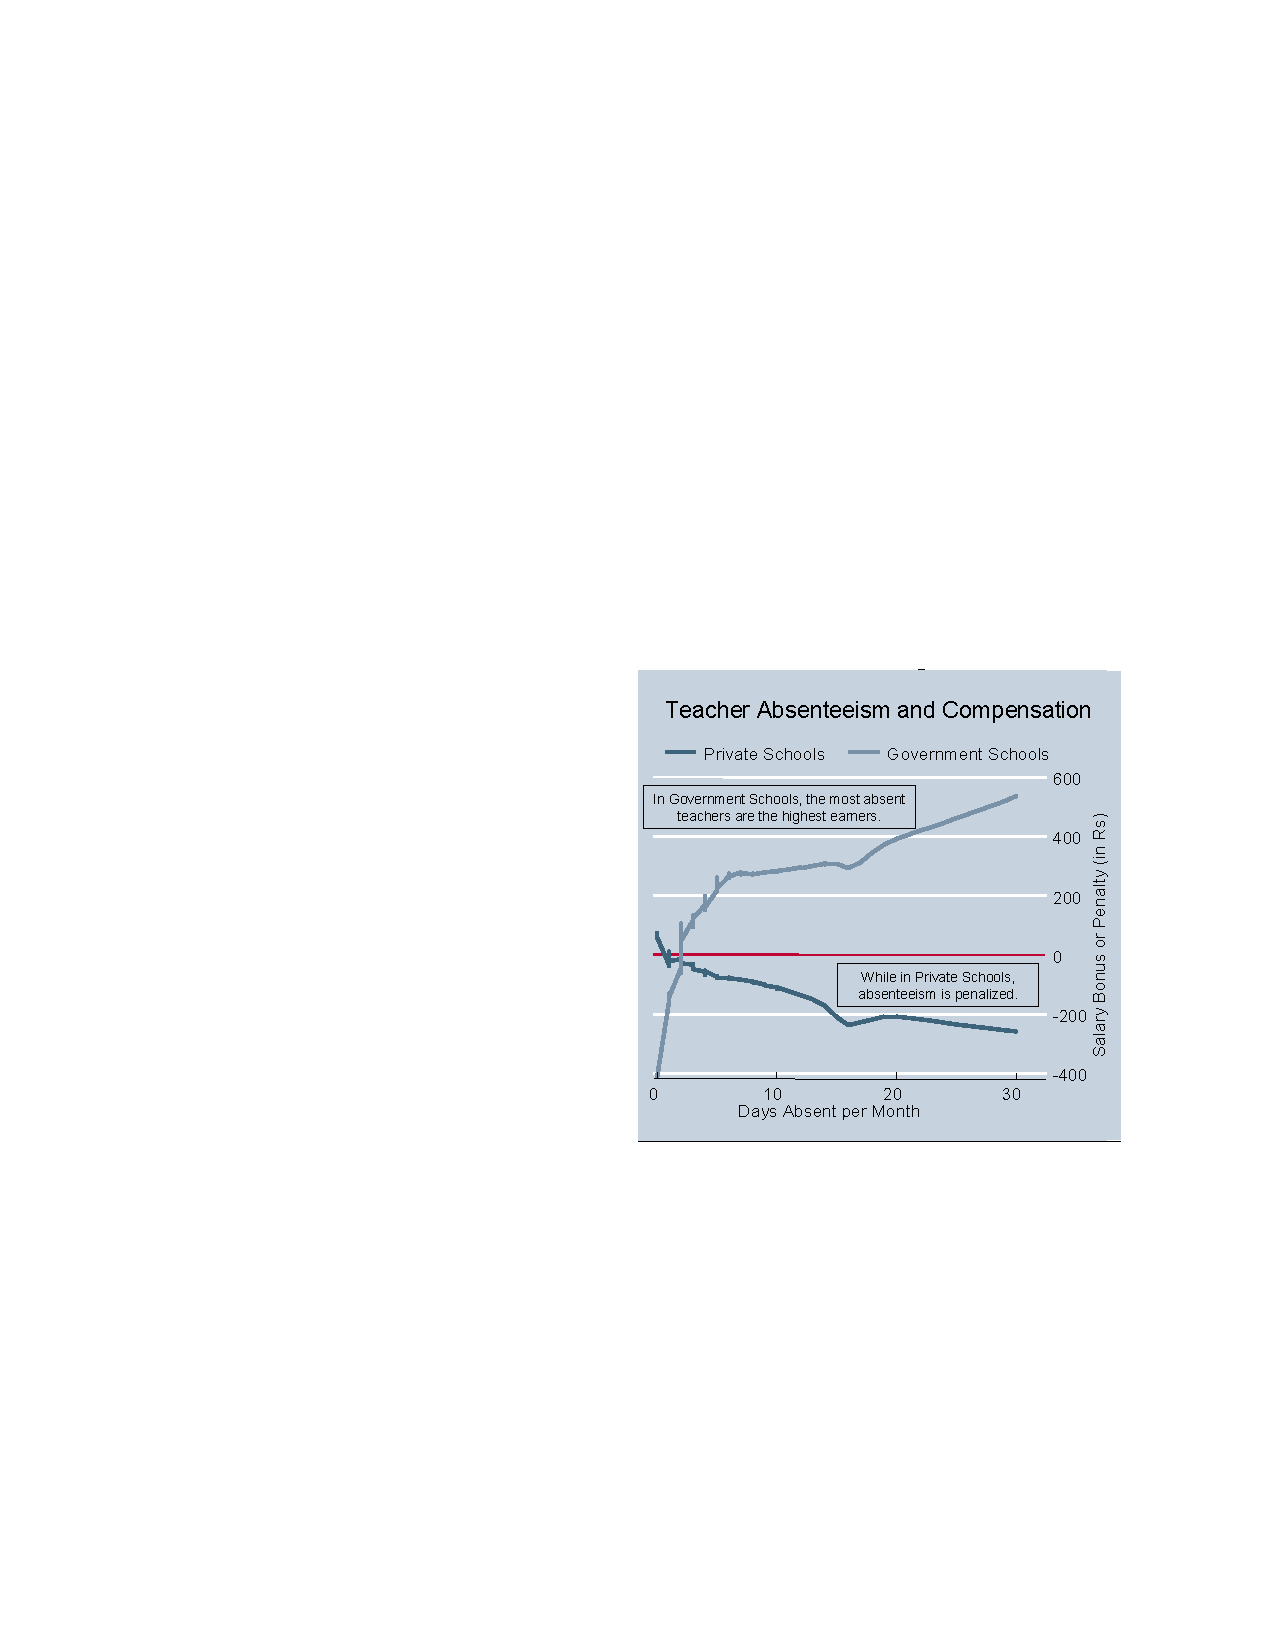
\includegraphics[scale=0.7]{graphs/absenteeism_and_pay.pdf} 
		\end{center}
	\end{figure}
\end{frame}

\begin{frame}{}
	\begin{figure}[htb]
		\begin{center}
			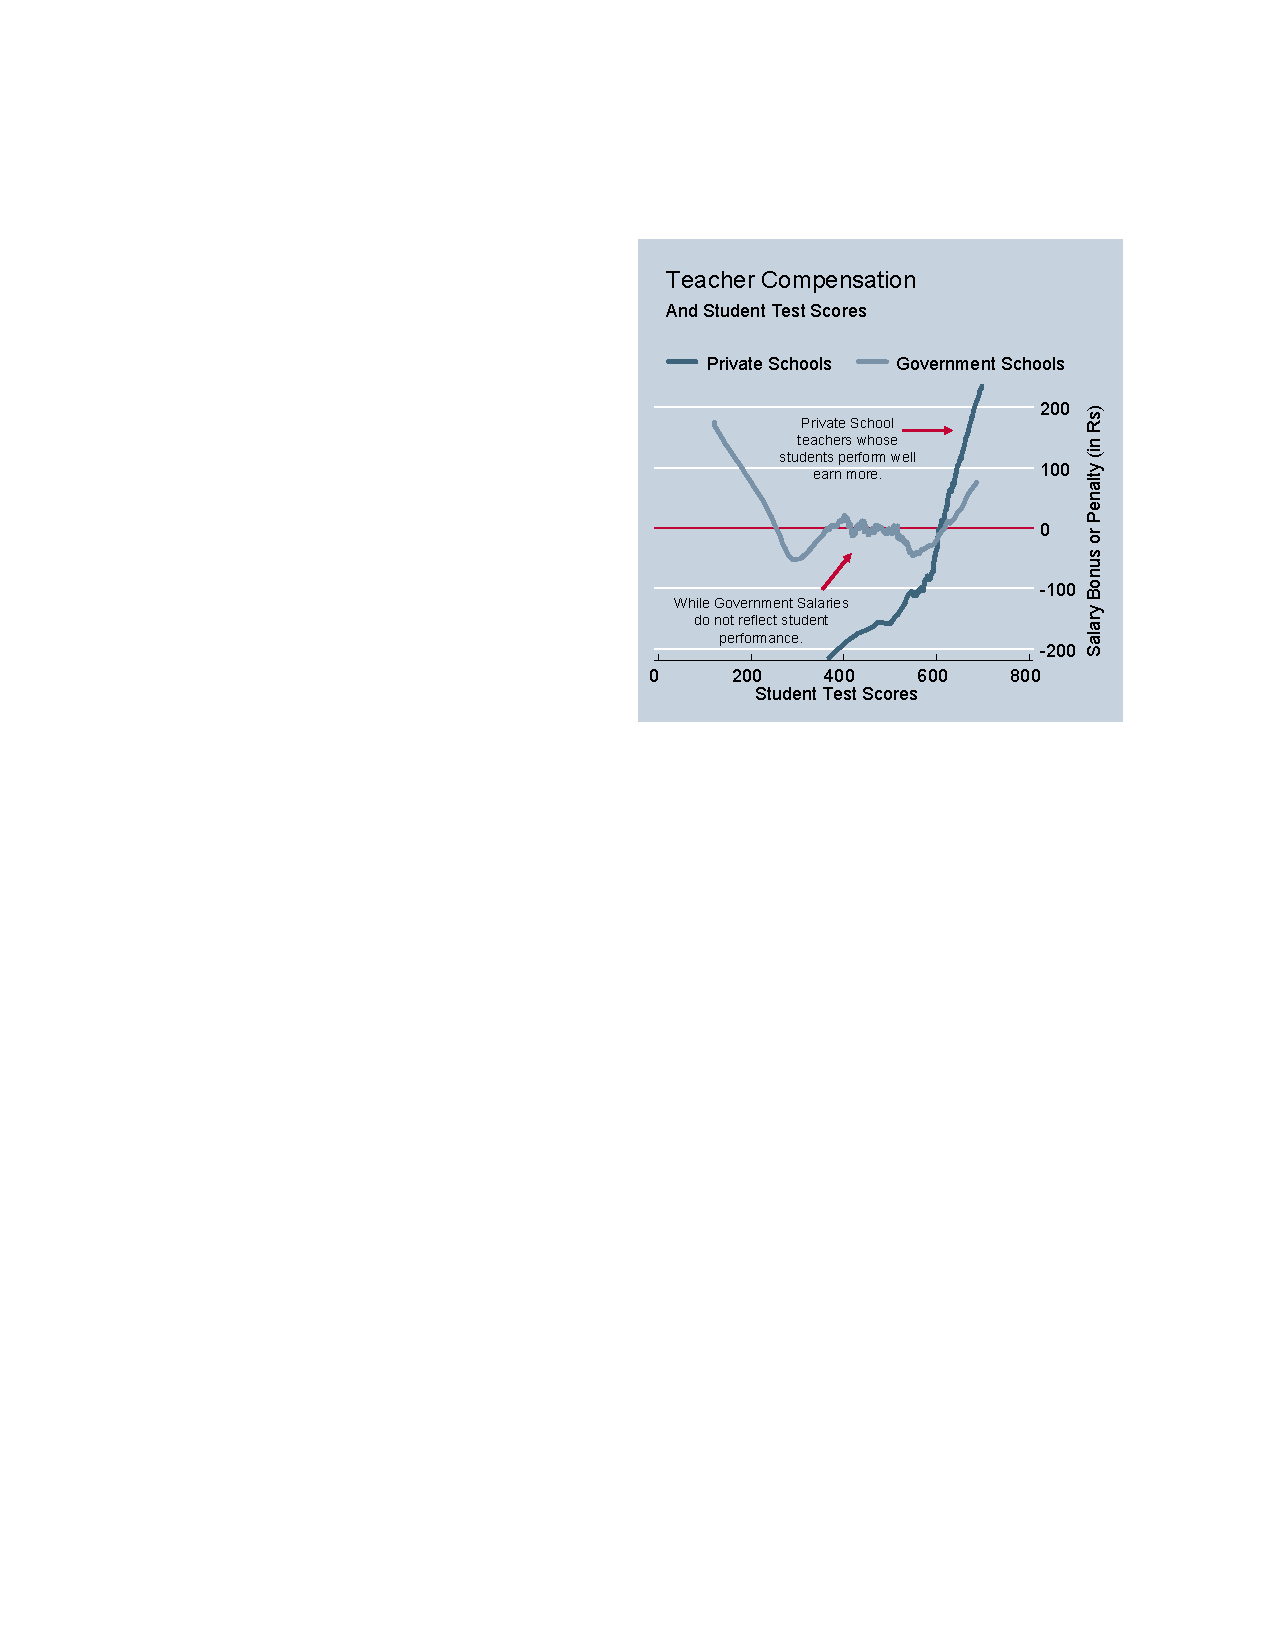
\includegraphics[scale=0.7]{graphs/compensation_scores.pdf}
		\end{center}
	\end{figure}
\end{frame}

\begin{frame}{No Difference in Incentives}
\begin{figure}[htb]
	\begin{center}
	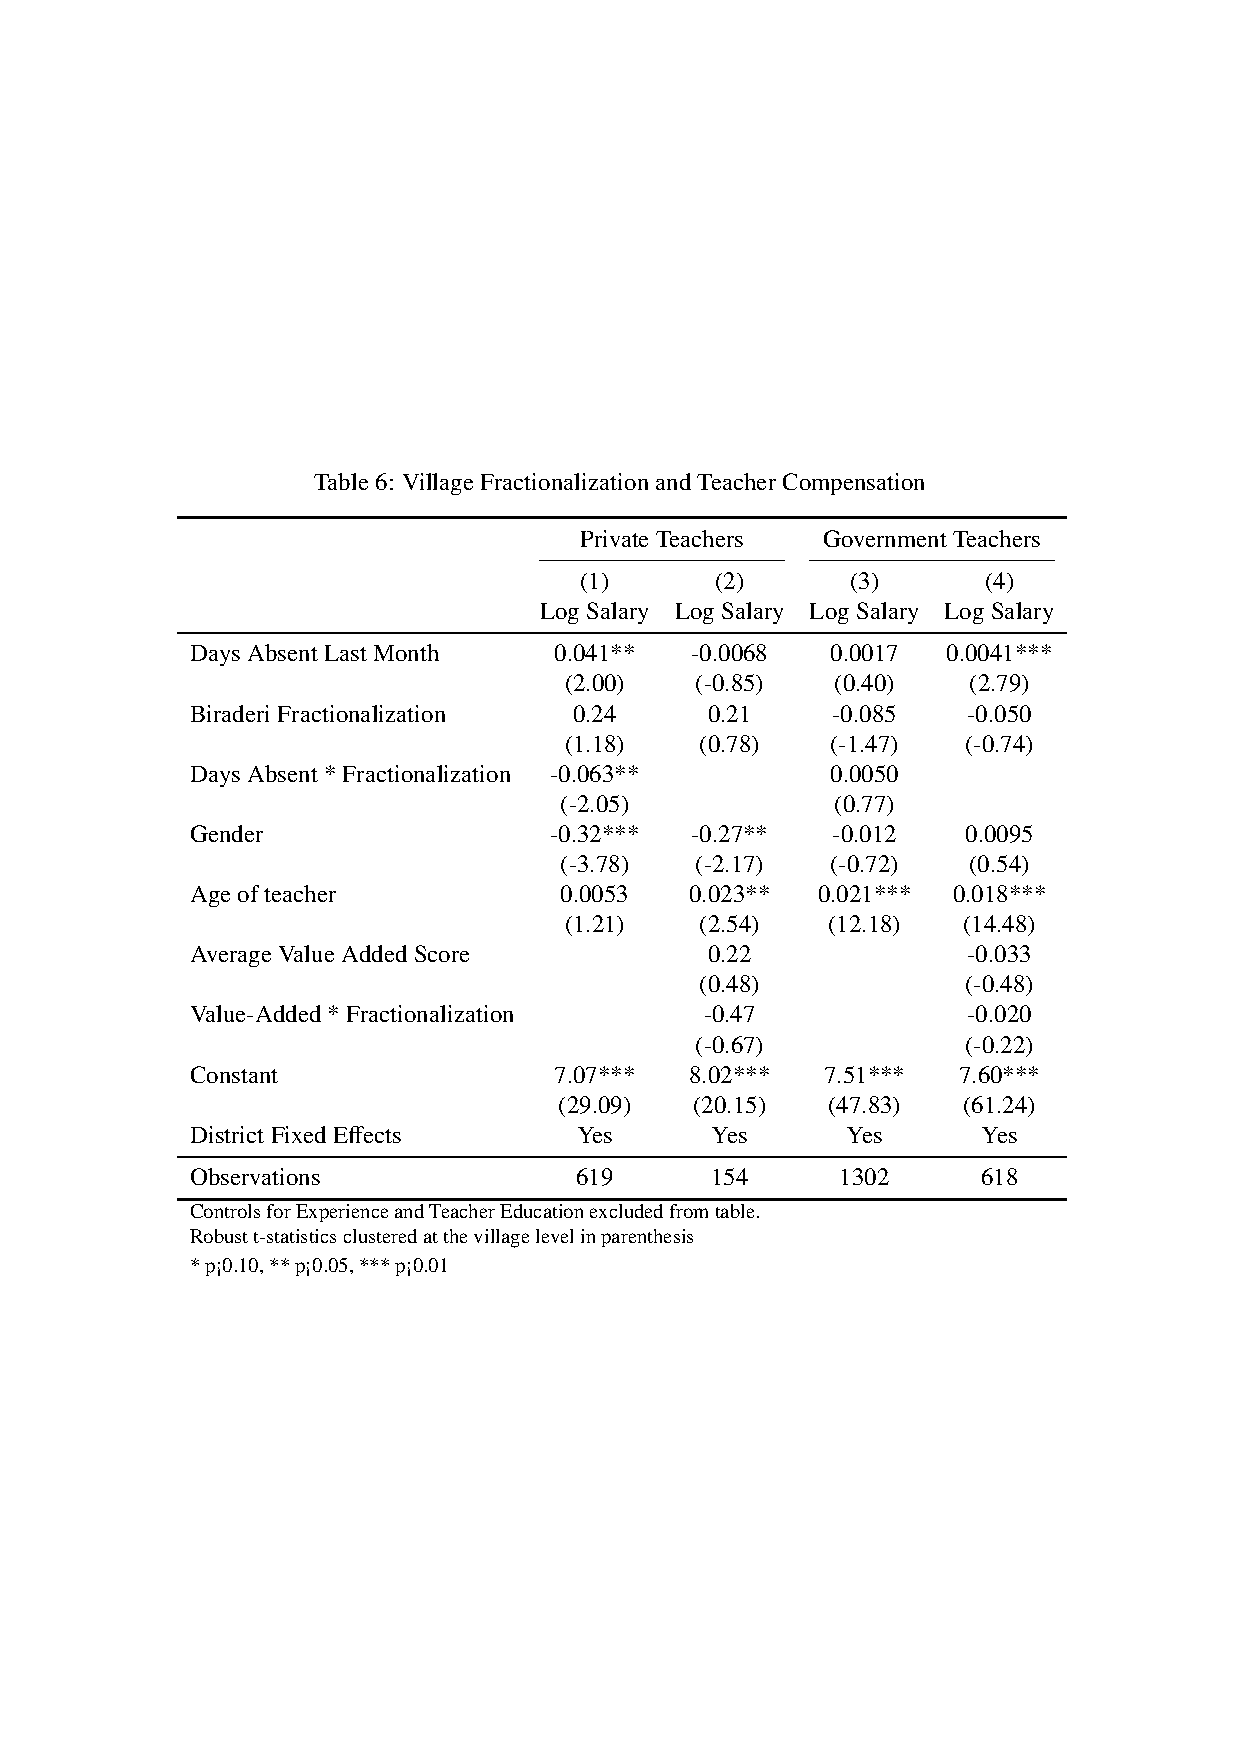
\includegraphics[scale=0.7]{tables/frac_and_compensation.pdf}
	\end{center}
\end{figure}
\end{frame}

\section{Selective Sorting}\label{}
\begin{frame}{Outline}
	\tableofcontents[currentsection]
\end{frame}

\begin{frame}{A Sorting Story}
	\begin{description}
		\item [Homogenous Villages:] Children sort on academic potential.
		\item [Fractionalized Villages:] Children also sort by social status.
	\end{description}
	\pause
	\begin{enumerate}
		\item Parents pick winners
	\end{enumerate}
\end{frame}

\begin{frame}{}
	\begin{figure}[htb]
		\begin{center}
		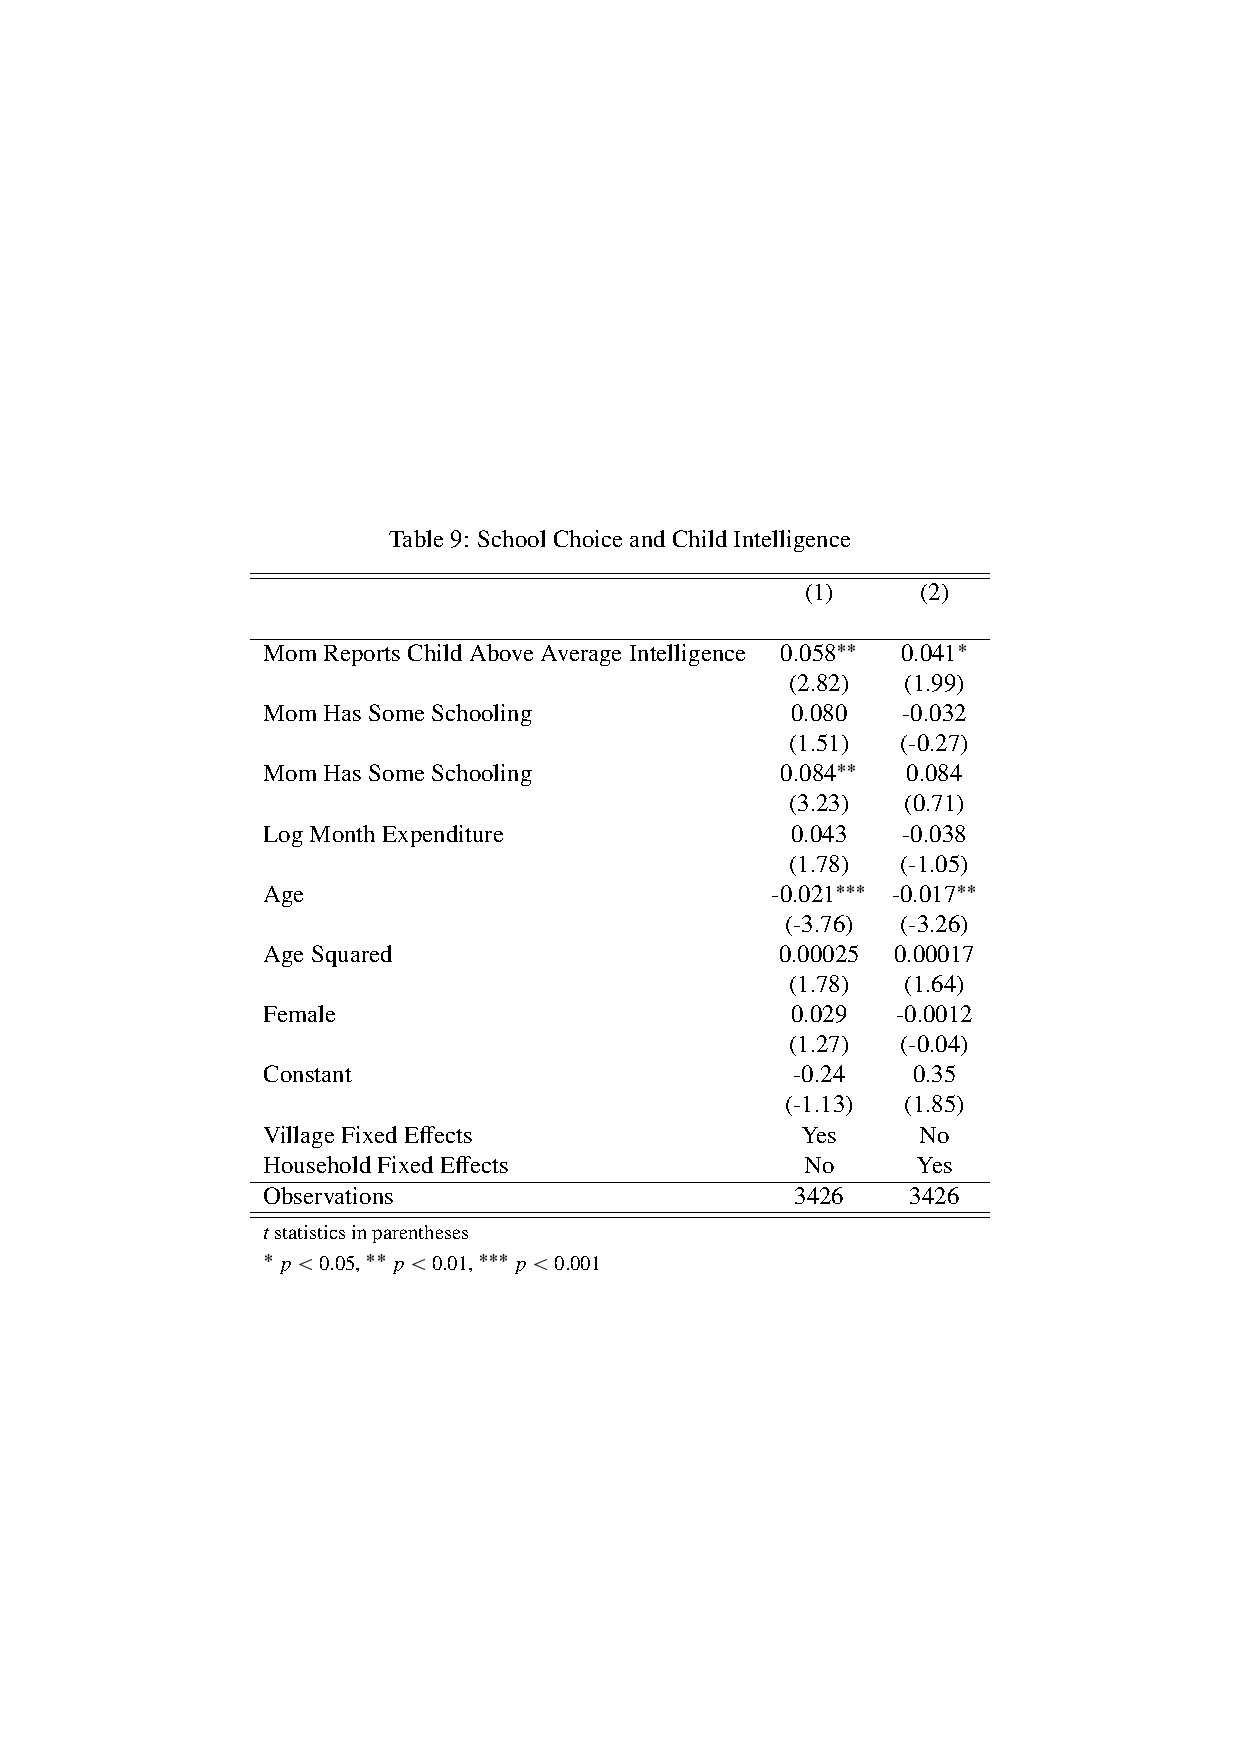
\includegraphics[scale=0.7]{tables/intelligence_type.pdf}
		\end{center}
	\end{figure}
\end{frame}

\begin{frame}{}
	\begin{figure}[htb]
		\begin{center}
		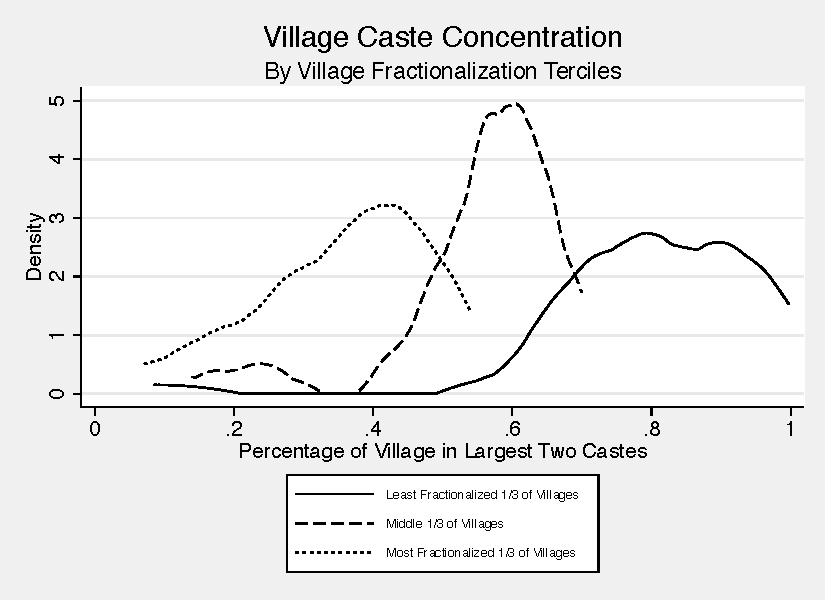
\includegraphics[scale=0.4]{graphs/village_toptwo.pdf}
		\pause \\
		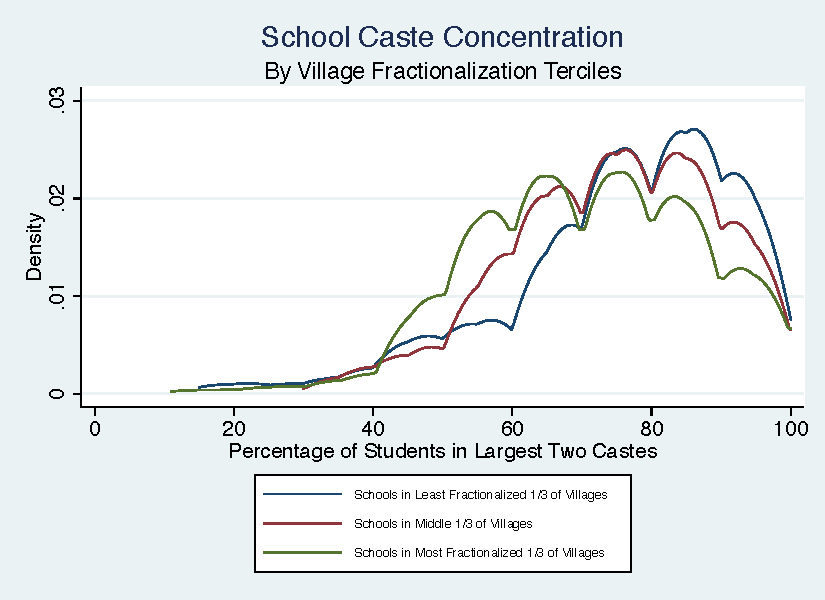
\includegraphics[scale=0.4]{graphs/school_toptwo.pdf}
		\end{center}
	\end{figure}
\end{frame}

\begin{frame}{}
	\begin{figure}[htb]
		\begin{center}		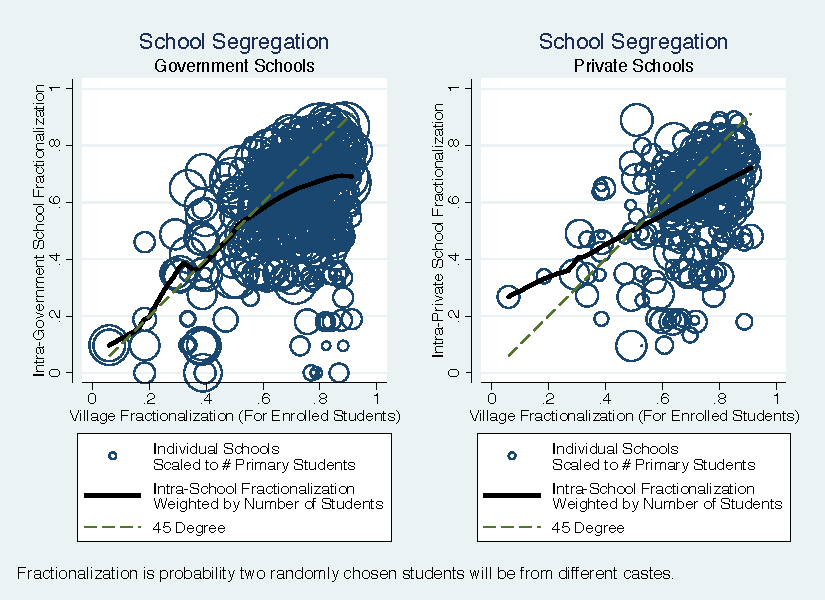
\includegraphics[scale=0.8]{graphs/intra_versus_intervillage_frac_combined.pdf}
		\end{center}
	\end{figure}
\end{frame}

\begin{frame}{Social Status and School Type}
	\begin{figure}[htb]
		\begin{center}
		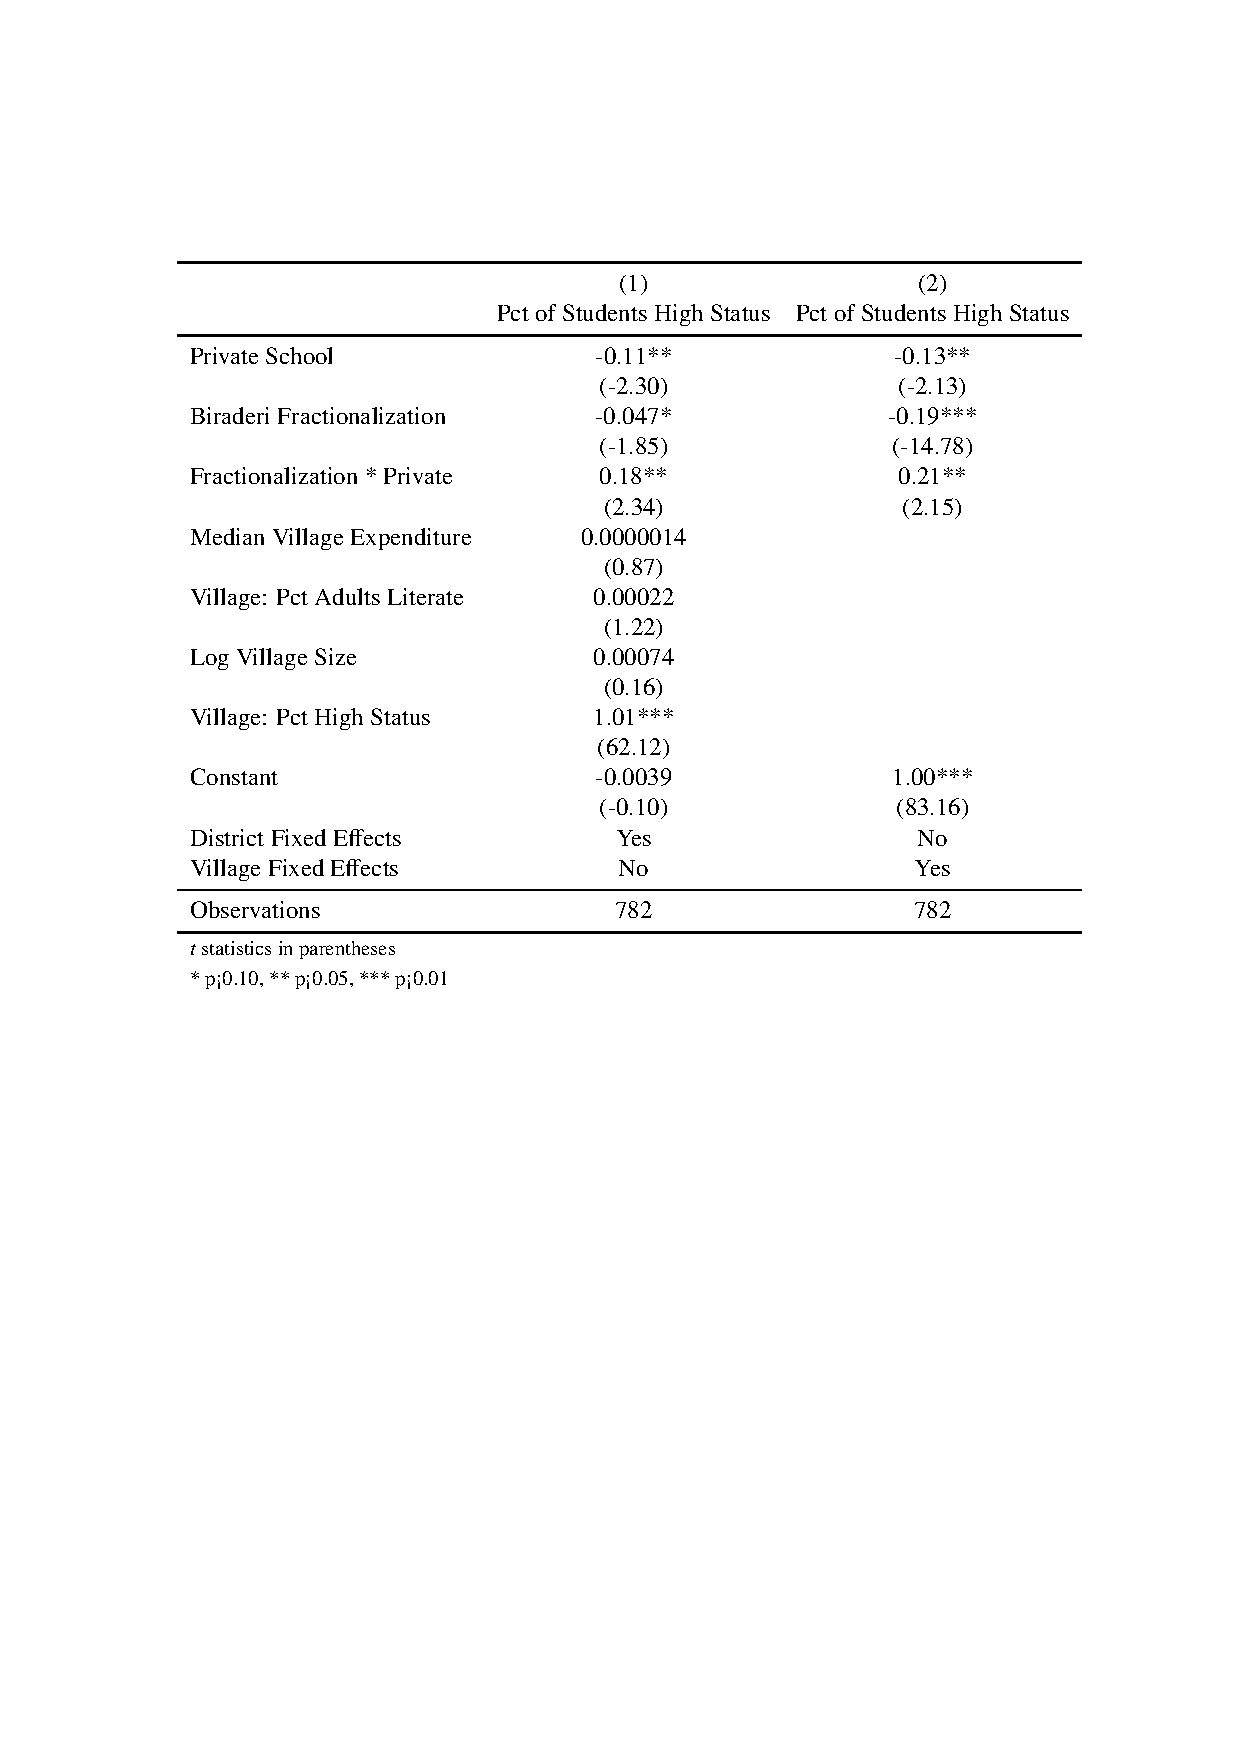
\includegraphics[scale=0.5]{tables/social_status_type.pdf}
		\end{center}
	\end{figure}
\end{frame}

\begin{frame}{Fractionalization and Prices}
	\begin{figure}[htb]
		\begin{center}
		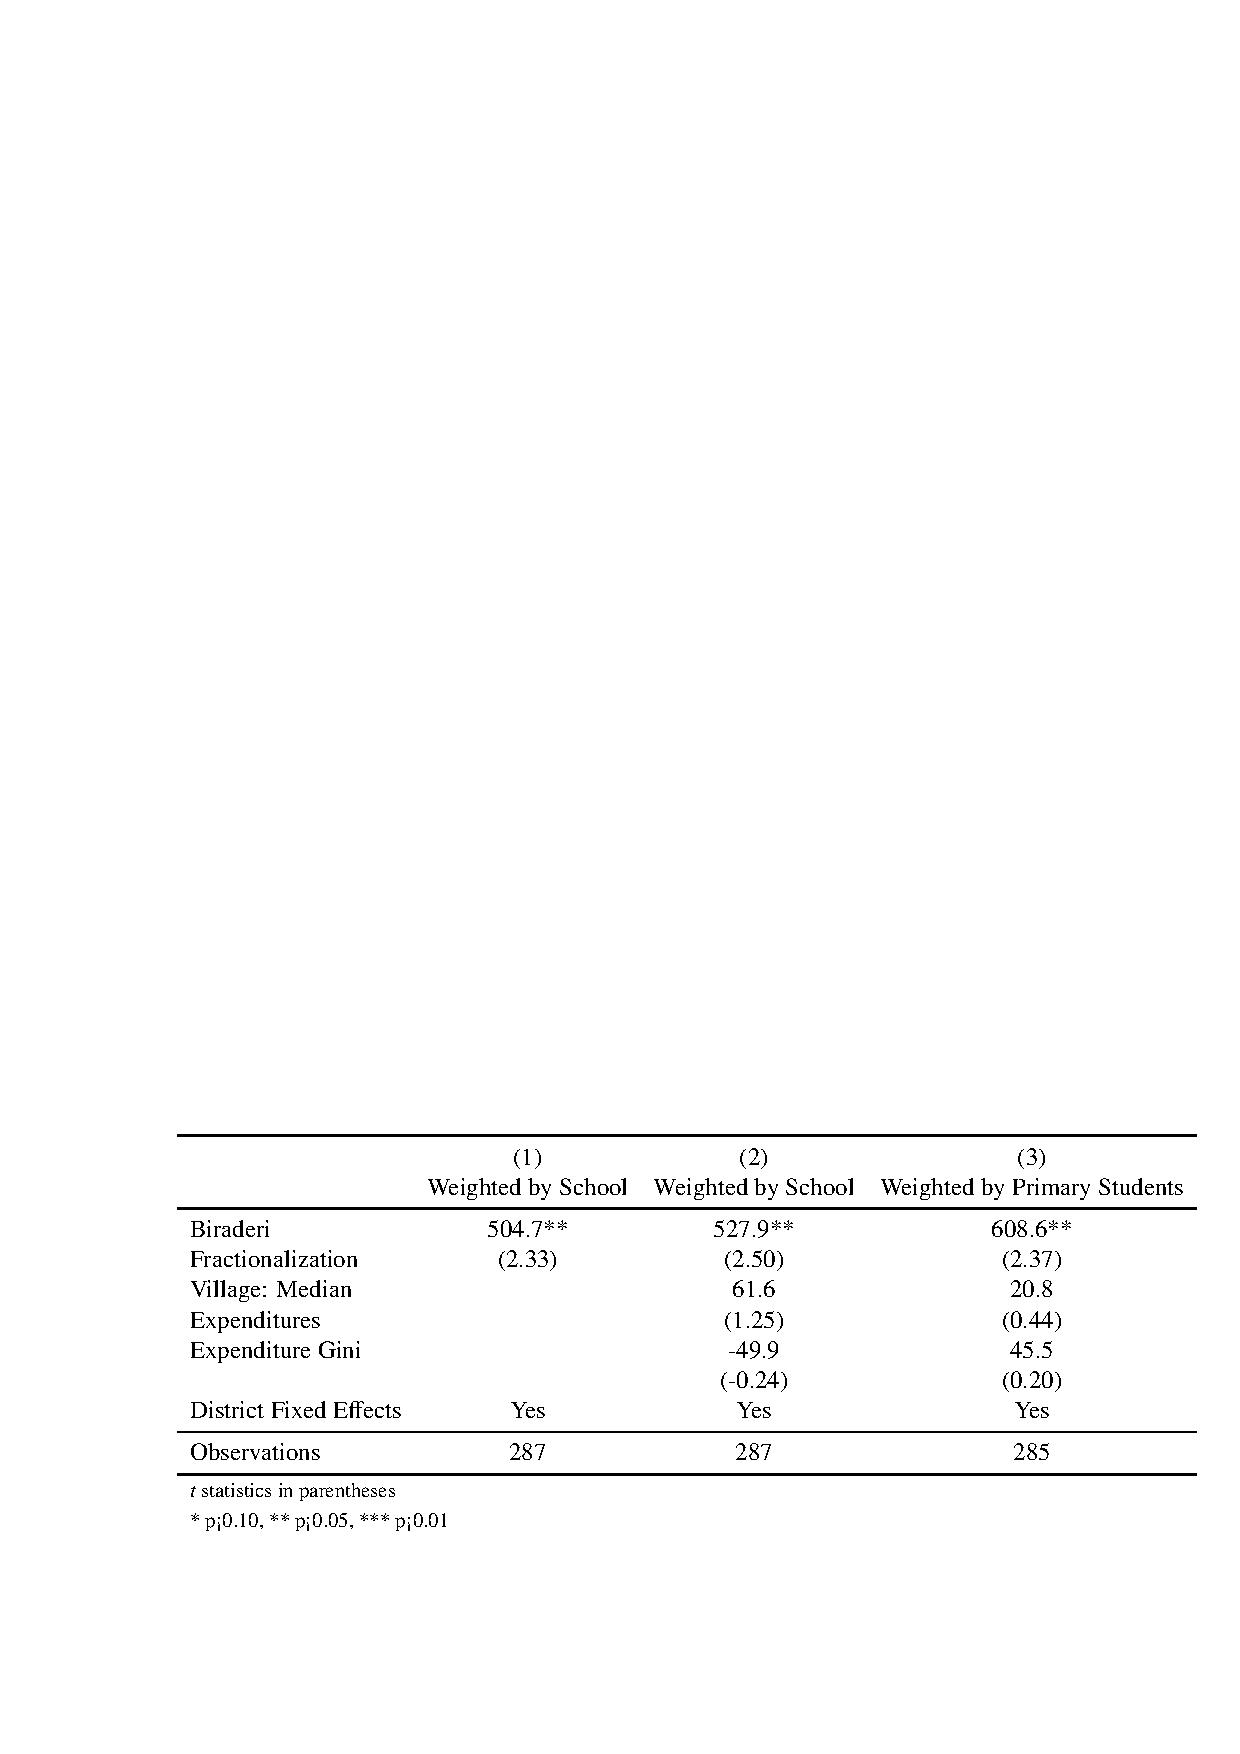
\includegraphics[scale=0.6]{tables/prices.pdf}
		\end{center}
	\end{figure}
\end{frame}

\begin{frame}{Sorting Paradox}
Why pay more for the same education?
\pause
\begin{description}
	\item [Neighborhood Effects:] Students performance is affected by peers
	\pause
	\item [Networking:] About forming positive associations. 
	\begin{itemize}
		\item In homogenous villages, most important association is intelligence.
		\item In fractionalized villages, caste matters too. 
	\end{itemize}
\end{description}
\end{frame}


\section{Discussion}\label{}
\begin{frame}{Outline}
	\tableofcontents[current]
\end{frame}


\begin{frame}{}
	Places a lower bound on role of sorting. 
\end{frame}
\end{document}